\newpage
\chapter{Trade-Off}
\label{ch-tradeoff}

%STICK TO THE STRUCTURE THAT IS INDICATED TO ENSURE CONSISTENCY, WE WILL BE WRITING THIS CHAPTER WITH MANY PEOPLE 

In this chapter, the various vehicle concepts are presented and elaborated upon. First of all, one has to acknowledge the distinction made between 3 groups or better yet, 3 capacity ranges, namely; 1-2, 4-6 and 20+ passenger vehicles. Each capacity range contains 3 vehicle concepts. The 3 vehicle concepts within the 1-2 passenger range are presented in \autoref{sc:1-2}, the 4-6 passenger vehicle concepts in \autoref{sc:4-6} and the 20+ passenger vehicles in \autoref{sc:20}. Furthermore, the complete trade-off is split up into two trade-offs. The first trade-off is the intermediate trade-off, in which the 3 concepts within a specific capacity range are traded off based on quantitative criteria such that only one concept is left per capacity range. The intermediate trade-off between the concepts within the 1-2 passenger range can be seen in \autoref{InterTO-12}, of the 4-6 in \autoref{InterTO-46} and of the 20+ passenger concepts in \autoref{InterTO-20}. In the final trade-off, the various capacity ranges along with their respective winner per capacity range (and their mission profile) are traded off based on both quantitative and qualitative criteria, and can be seen in \autoref{Sec:FinalTO}. To finalise this chapter, a risk analysis was performed and can be found in \autoref{sc:RiskAnalysis}.   


%In this chapter, an overview of the trade-offs of the concepts will be presented. First of all, a set of concepts in three different passenger range categories will be created; namely the 1-2, 4-6, and 20 plus passenger ranges. A preliminary trade-off of these concepts using only the quantitative parameters will be performed, in order to choose a winning concept for each passenger range that will move on to the final trade-off. The preliminary trade-off will be done by comparison of a selection of key numerical outputs using the criteria tool. The final trade-off follows the preliminary one, which will evaluate the full set of quantitative and qualitative parameters of the concepts, in order to choose the winning concept and with it, its specific mission profile. The final trade-off will make use of the trade criteria defined in \autoref{CriteriaTools}, including the weighting factors.  REFER TO SPECIFIC SECTIONS (FINAL TRADE-OFF) SIMONE.


\section{1-2 Passenger Vehicles}
\label{sc:1-2}
%Give a little introduction to 1-2 passenger vehicles 
A broad range of 1-2 passenger vehicle concepts are currently in existence. However, most of these designs are not commercially feasible, for example due to the fact that they are unsafe, aesthetically unpleasing or the choice of material is not sustainable. By having taken the commercial feasibility of the design into account while brainstorming about the vehicle, three new concepts were defined of which the sketches are presented in \autoref{1-2A}, \autoref{1-2B} and \autoref{1-2C}. The concepts are evaluated by using the integrated tool which was introduced in \autoref{sec:Tools}. In \autoref{InterTO-12} the intermediate trade-off for this vehicle capacity is performed, based on the quantitative outputs of the tools.  

%While brainstorming with the commercial feasibility of the design taken into account, three new concepts were defined. The drawings of these concepts are presented in \autoref{1-2A}, \autoref{1-2B} and \autoref{1-2C}.

\subsection{Concept Definition}
\label{1-2Concepts}
%Include figures and descriptions of vehicles, plus parameters that will go into the tool 

\begin{figure}[H]
  \centering
  \begin{minipage}[b]{0.25\textwidth}
    \includegraphics[width=5.0cm]{./Figures/Concept12a.png}
    \captionsetup{justification=centering}
    \caption{Concept 2A}
    \label{1-2A}
  \end{minipage}
  \hspace{1.5cm}
  \begin{minipage}[b]{0.30\textwidth}
    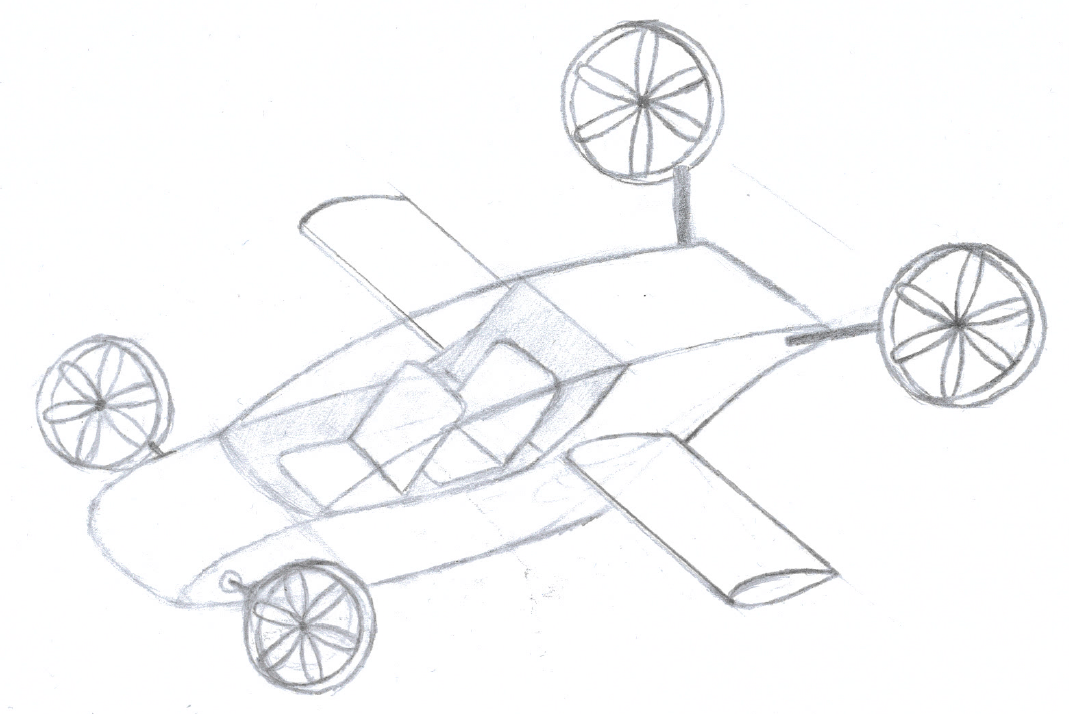
\includegraphics[width=5.0cm]{./Figures/Concept12b.PNG}
    \captionsetup{justification=centering}
    \caption{Concept 2B}
    \label{1-2B}
  \end{minipage}
  \hspace{0.5cm}
  \begin{minipage}[b]{0.25\textwidth}
    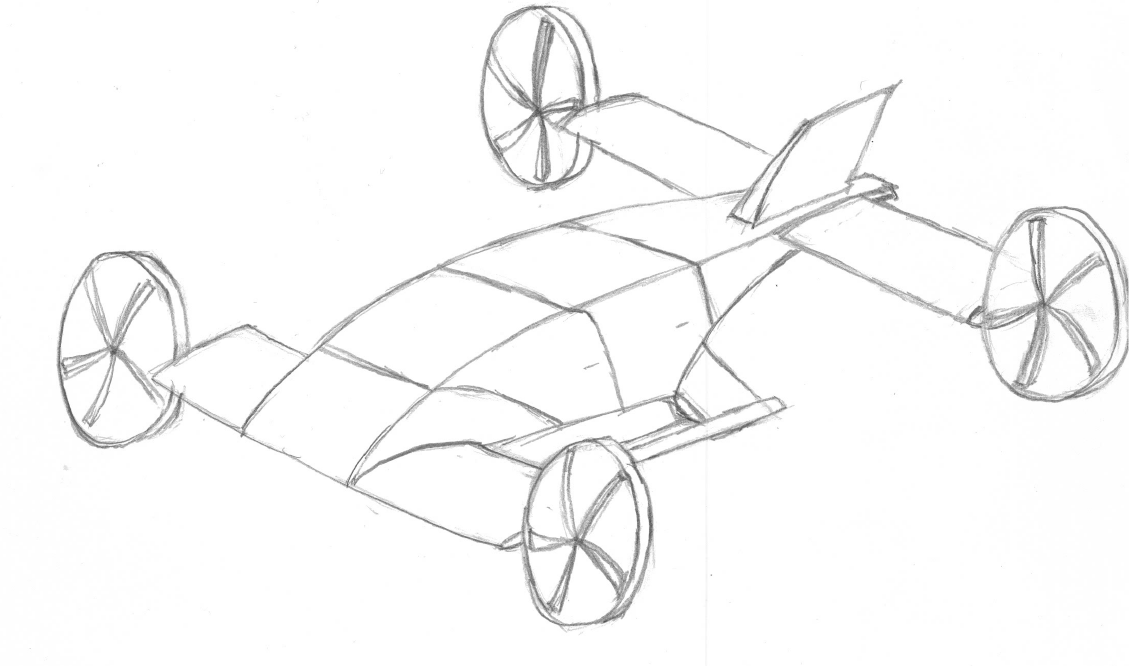
\includegraphics[width=5.0cm]{./Figures/Concept12c.PNG}
    \captionsetup{justification=centering}
    \caption{Concept 2C}
    \label{1-2C}
  \end{minipage}  
\end{figure}

\paragraph{Concept 2A}
Concept 2A is in essence a flying wing with a fan located in front of the cockpit, a set of fans located in the wing and a set of fans located on top of the wing next to the fuselage as seen in \autoref{1-2A}. The fan located in the front is a coaxial ducted fan and is solely used for vertical take-off and landing, after which the latches close for the cruise configuration. The set of fans located in the wing are used for vertical take-off and landing, and are rotated $90\degree$ for the cruise configuration to produce thrust. One should acknowledge that the fans as seen in \autoref{1-2A} do not represent the final vehicle concept, as the wing only contains one (bigger) fan per half span, rather than 4 rotors per half span. The fans located on top of the wing pivot around the trailing edge of the wing and are fully horizontal in VTOL configuration. These fans are used to produce thrust during cruise, as seen in the configuration shown in \autoref{1-2A}. Furthermore, the passenger seating arrangement is side-by-side and the passengers will enter the vehicle from the sides.

\paragraph{Concept 2B}
This particular concept has a narrow body with one wing, which naturally produces lift during cruise to improve the cruise performance. Furthermore, it has four tilt-able rotors of which the ones in the back have a slightly larger diameter compared to those in the front to account for the expected slightly aft centre of gravity position resulting in the rotors in the back having to take up a higher percentage of the MTOW during VTOL than those in the front. All rotors are used during VTOL in which all are in the fully horizontal position and during cruise, the rotors in the back are in fully vertical position, whereas the ones in the front are angled in order to produce thrust and lift simultaneously. To finish off this concept, the passengers are seated behind one another and will be able to enter the vehicle from the side.

\paragraph{Concept 2C}
The configuration of concept 2C is composed of front and rear wing surfaces, with tilt rotors at the tips of all the wing surfaces. These rotors therefore tilt horizontally to provide hover propulsion, which is when they are used at their maximum power output. During cruise, all rotors tilt vertically to provide horizontal propulsion, with the wing surfaces providing lift force to the vehicle. The rotors measure approximately 1.7 meters in diameter, making them relatively large, while consequently making the total width large, and therefore space demanding. This also induces large tip loads on the wing structure which will require a lot of structural reinforcement efforts. The seating configuration is one behind the other, which satisfies the width minimisation required due to large tip rotors and wing surfaces. The users would enter the vehicle from the side through doors placed on the side that open vertically.  

% iPce. elease add the foe vehllowing required packages to your document preamble:
% \usepackage{booktabs}
\begin{table}[H]
\captionsetup{justification=centering}
\caption{Input of tools for 1-2 person vehicle}
\label{12input}
\begin{tabular}{@{}llll@{}}
\toprule
\textbf{Parameter}                       & \textbf{Concept 2A} & \textbf{Concept 2B} & \textbf{Concept 2C} \\ \midrule
MTOW {[}kg{]}                            &           634         &        575           &         667           \\
OEW/MTOW           &          0.45          &         0.40          &             0.47       \\
\# Passengers {[}-{]}                    &          2          &         2           &             2       \\
Range {[}km{]}                           &          60          &         60     &            60        \\
Max Dimension {[}m{]}                    &         5.75           &          5          &            6        \\
%Battery Energy density {[}Wh/kg{]}       &           260         &       260  &            260        \\
%Battery Power density {[}W/kg{]}         &           2100         &      2100 &            2100        \\
L/D {[}-{]}                              &           17         &        12            &           16         \\
Radius of rotors (x number of rotors) &   0.75 (1x) \& 0.4 (2x) \& 0.5 (2x)                &    0.85 (2x) \& 0.8 (2x)&            0.85 (x4)       \\
Cruise Velocity {[}m/s{]}                &          42          &        32            &            37        \\ \bottomrule
\end{tabular}

\end{table}


\subsection{Intermediate Trade-off}
\label{InterTO-12}
%Present the outputs of the tools for each option, put it in a table and discuss which 1 (or 2) is best. Explain that we will continue with that one to the final trade off, where we will investigate that option further by looking at additional qualitative factors like user experience, passenger comfort, safety etc..   

The inputs that were mentioned in \autoref{1-2Concepts} were put into the criteria tools. The main results are tabulated in \autoref{12output} and the values for the criteria are scaled into scores between 1 and 5 and are used in the intermediate trade-off.  

% \begin{table}[H]
% \centering
% \captionsetup{justification=centering}
% \caption{Output of tools for 1-2 person vehicle}
% \label{12output}
% \begin{tabular}{@{}llll@{}}
% \toprule
% \textbf{Parameter}                           & \textbf{Concept 2A} & \textbf{Concept 2B} & \textbf{Concept 2C} \\ \midrule
% \# Vehicles {[}-{]}                          &         9800          &        12900        &           11200         \\
% \# Pads {[}-{]}                               &       1570           &    1620      &  1610  \\
% \# Trips/day {[}-{]}                         &          283000          &     308000          &           294000         \\
% \#  Payload Range Energy Efficiency          &          0.0305          &       0.0352     &        0.0304      \\
% \# Ticket price {[}\$/km{]}                  & 2.86                   & 2.34                   & 3.04                    \\
% \# Ticket price {[}\$/km-pad costs{]}        & 0.64                    & 0.62                   & 0.65                   \\
% \# Passengers/day {[}-{]}                    &          305000          &     327000        &           314000        \\
% Vertiport Area {[}m\textsuperscript{2}{]}    &          760          &      630        &           830      \\
% Total System Area {[}km\textsuperscript{2}{]} &          1.19         &     1.01  &         1.34         \\
% Total Board Time {[}s{]}                     &          210          &     210               &               210     \\
% Noise {[}dBA{]}                              &             82       &     71          &           73        \\
% Downwash {[}m/s{]}                              &             51       &     34          &           36        \\ 
% Maximum Hub Throughput [vehicles/hour]      & 14414  & 16389 & 15026 \\ \bottomrule
% \end{tabular}
% \end{table}

\begin{table}[H]
\centering
\captionsetup{justification=centering}
\caption{Output of tools for 1-2 person vehicle}
\label{12output}
\begin{tabular}{@{}llll@{}}
\toprule
\textbf{Parameter}                                          & \textbf{Concept 2A} & \textbf{Concept 2B} & \textbf{Concept 2C} \\ \midrule
\# Vehicles                                                 &     9800       &      12900      &    11200        \\
\# Payload Range Energy Efficiency  {[}-{]}                         &      0.0305      &  0.0352          &  0.0304          \\
\# Ticket price {[}\$/km-pad costs{]}                        &     0.64       &  0.62          &     0.65       \\
\# Passengers/day {[}-{]}                                   &     305000       &    327000       &   314000         \\
Total System Area {[}km\textsuperscript{2}{]}                  &    1.19        &    1.01        &    1.34        \\
Noise {[}dBA{]}                                             &     82       &       71     &      73      \\ 
Downwash {[}m/s{]}                                          & 51            & 34            & 36        \\ \bottomrule
\end{tabular}
\end{table}

Table \ref{12criteriascores} below shows the resultant quantitative criteria scores of the three different vehicle concepts.

\begin{table}[h]
\centering
\captionsetup{justification=centering}
\caption{Criteria scores for 1-2 person vehicle}
\label{12criteriascores}
\begin{tabular}{@{}llllll@{}}
\toprule
\textbf{Group}                           & \textbf{Criteria}  & \textbf{Criteria Weight}  & \textbf{2A}   & \textbf{2B}   & \textbf{2C}   \\  \midrule
\multirow{2}{*}{Ecologic Sustainability} & PREE & 0.278                   & 5             & 5             & 5             \\
                                         & Battery mass       & 0.078                   & 5             & 4             & 4             \\\midrule
\multirow{2}{*}{Social Acceptance}       & Noise              & 0.258                   & 3             & 5             & 5             \\
                                         & Downwash           & 0.055                   & 4             & 5             & 5             \\\midrule
Cost/Profit                              & Ticket price       & 0.189                   & 2             & 2             & 1             \\\midrule
Technical Risk                           & ATM/UTM efforts    & 0.140                   & 3.25          & 1.42          & 2             \\  \midrule
\textbf{}                                & \textbf{}          & \textbf{Weighted Score} & \textbf{3.61} & \textbf{3.85} & \textbf{3.74}  \\ \bottomrule
\end{tabular}
\end{table}


As shown by the final weighted score of the concepts against the criteria, concept 2B has shown to be the most optimal concept for the 1-2 passenger vehicle capacity. From the table of parameters, \autoref{12output}, it can be seen that concept 2B scored best in terms of energy efficiency, ticket price per km, total system area and noise level. Concept 2C produced similar numbers, however it has a significantly smaller PREE of 0.0304 compared to 0.0352 of concept 2B. Concept 2A has a noise level of 82 dBA, which is considered to be too high and has excessive down wash, making it less favourable against the highly weighted social acceptance criteria. Hence concept 2B presents itself as the best concept and moves on to the final trade-off in \autoref{Sec:FinalTO}. 



\section{4-6 Passenger Vehicles}
\label{sc:4-6}
%Give a little introduction to 4-6 passenger vehicles 
The range of 4-6 passengers is an interesting market for urban air mobility as it has the user experience of a taxi in the air. Lately, Lilium launched their five passenger vehicle \footnote{\url{https://lilium.com/the-jet} [accessed 21-05-19]} and multiple other vehicle concepts in this passenger range already have been proposed. At the end of the section, one 'winner' will be selected to investigate further and compare to the best concepts for the other vehicle capacities (\autoref{InterTO-46}). 

\subsection{Concept Definition}
%Include figures and descriptions of vehicles, plus parameters that will go into the tool. 
Based on research into existing air taxi concepts, the majority of well-developed vehicles fall into 3 categories. As an initial trade-off, one vehicle from each of these categories is considered. In each case, the OEW/MTOW (not including the battery mass) is set at a specific ratio. This is done to prevent unrealistic designs. The effect of this choice will be considered in the sensitivity analysis. During the design process for the 4-6 vehicles, different sensitivity analyses were done to come up with the best capacity for each vehicle. Other than that, the speed and ranges are adjusted during the design phase to find the optimal parameters. 

\paragraph{Concept 1: The Electric Jet}
The first vehicle considered is called the "Electric Jet" (\autoref{4-6A}), and is similar to the Lilium Jet\footnote{\url{https://www.lilium.com} [accessed 21-05-19]}. It features fixed wings in a canard configuration with small electric turbines located along the trailing edges of the wings. While this vehicle is designed for highly efficient and low-drag forward flight, it also has very high disk loading in hover and takeoff. During market analysis, it was found that there is little demand for long duration journeys, so a scaled 4 passenger version is presented for trade-off. The passengers sit 2x2 and board from both sides of the vehicle.

\paragraph{Concept 2: The Tilt-Wing}
Another concept category is the Tilt-wing, as depicted in \autoref{4-6B}. This concept has 4 large propellers mounted on forward swept tilt-wings. When the wings tilt up for takeoff and landing, the rotors raise up, and provide safe clearance. A canard wing and nose rotors are also needed for balance in hover. A pusher fan (or two) is also attached at the stern for use in forward flight. From statistics, winged aircraft gain significant efficiency advantage in forward flight, and also can attain higher speeds. The passengers sit 2x2 and board from one side. This concept will allow for a bit more forward space than the electric jet in order to accommodate boarding.

\paragraph{Concept 3: The Gondola}
In \autoref{4-6C} a vehicle design for six passengers can be seen. The vehicle looks like a gondola. There are two benches in the vehicle on which three people can sit per bench. On top of the vehicle, four coaxial rotors are placed. The four coaxial rotors will placed outwards from the cabin of the vehicle to ensure that minimal interaction between the cabin and downwash takes place, which in general translates into a better lift production and a reduction in noise in the cabin. The landing gear is designed as a wheel within a box, with the wheel retracting from the box during taxiing. These structures are placed on each corner of the vehicle and as can be seen in the figure there is room under the benches fof battery storage. 

%They will be placed outwards of the vehicle to make sure that the rotors will produce a better lift. Next to that, the rotors should be placed as much as possible outwards to prevent the interference of noise with the vehicle.

\begin{figure}[H]
  \centering
  \begin{minipage}[b]{0.25\textwidth}
    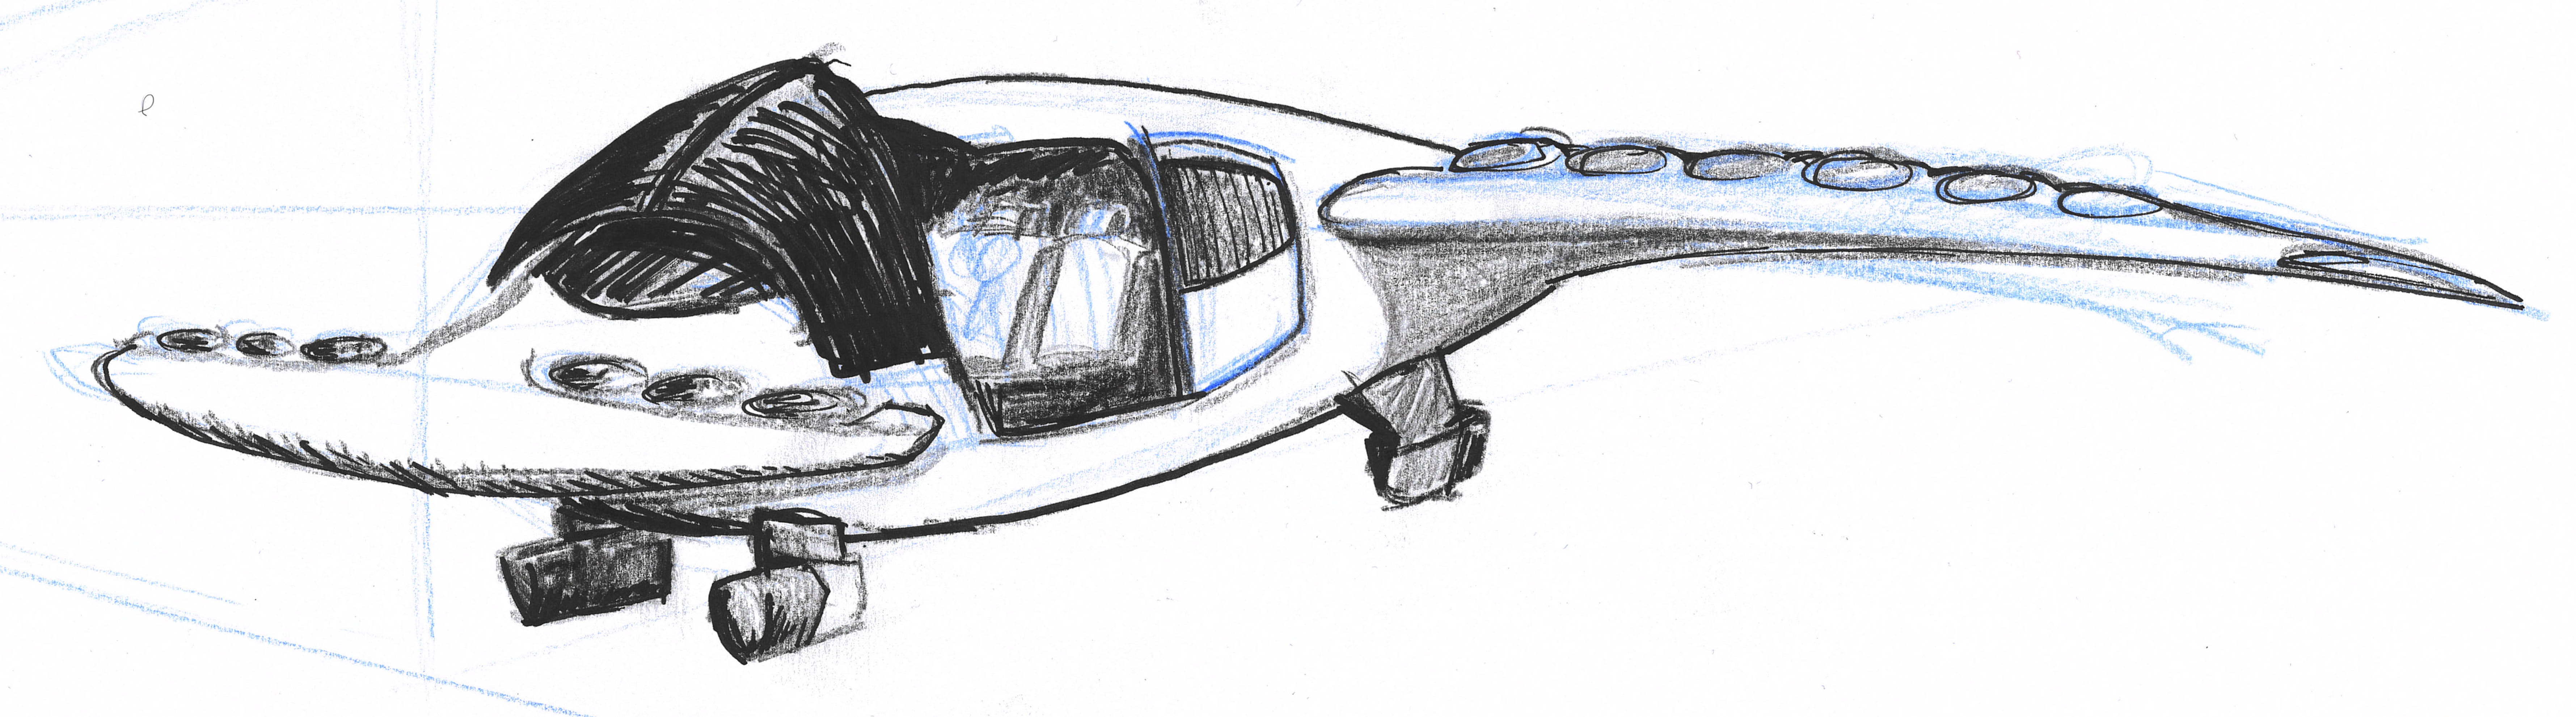
\includegraphics[width=5.0cm]{./Figures/ejet.jpg}
    \captionsetup{justification=centering}
    \caption{Electric Jet 4}
    \label{4-6A}
  \end{minipage}
  \hspace{1.5cm}
  \begin{minipage}[b]{0.30\textwidth}
    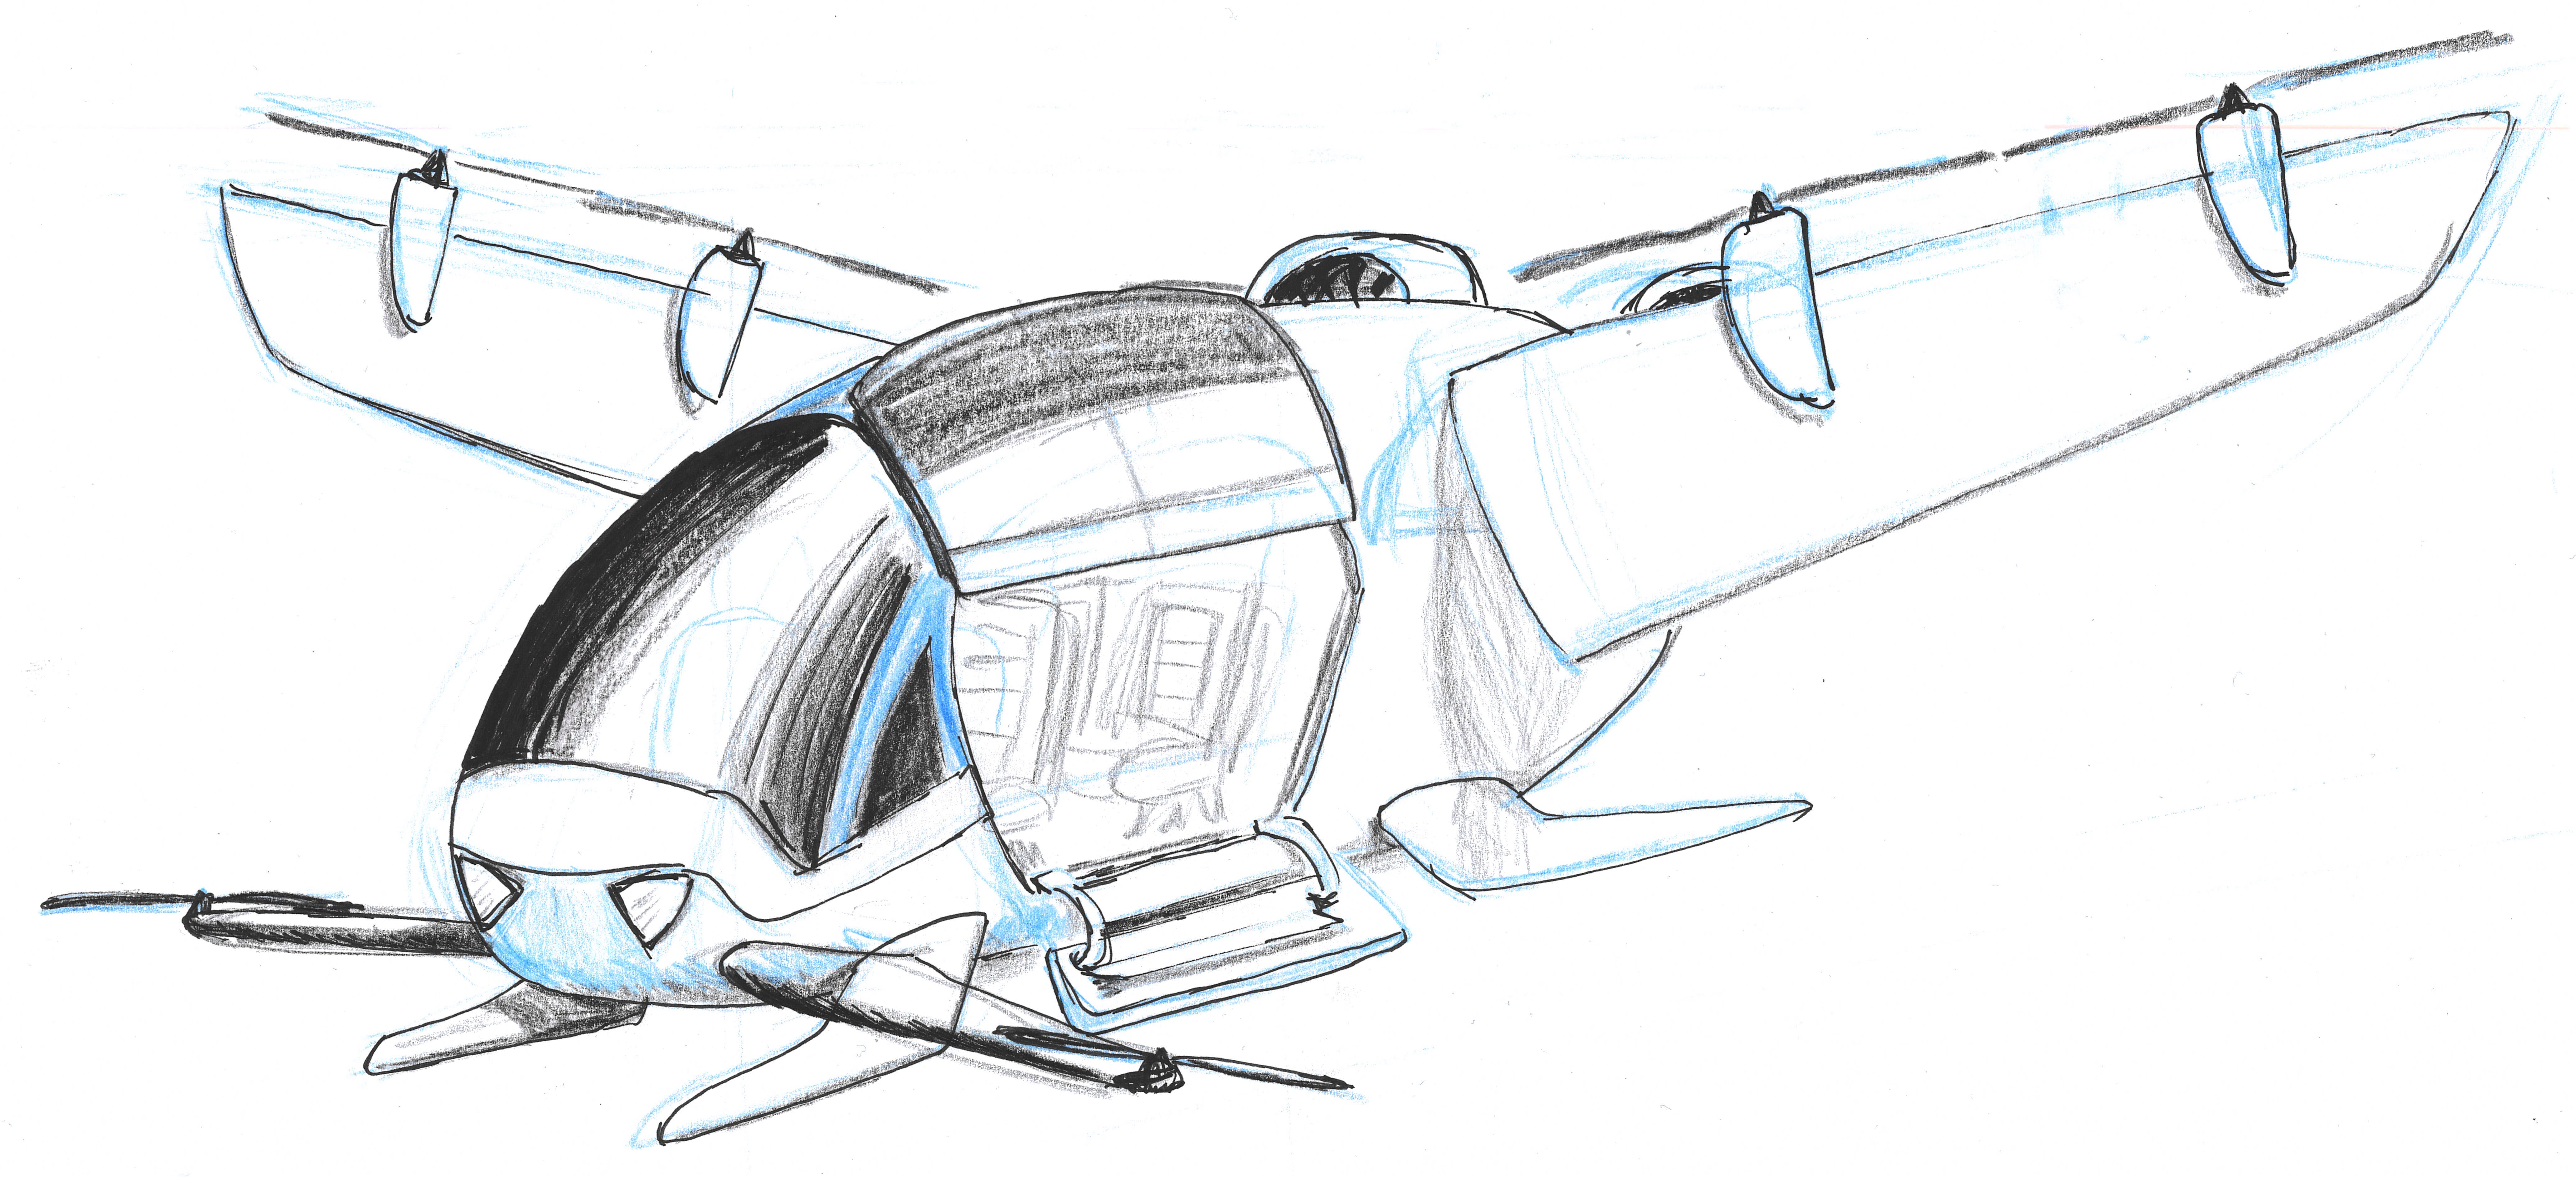
\includegraphics[width=5.0cm]{./Figures/bumblebee.jpg}
    \captionsetup{justification=centering}
    \caption{Tilt-wing 4}
    \label{4-6B}
  \end{minipage}
  \hspace{0.5cm}
  \begin{minipage}[b]{0.25\textwidth}
    \includegraphics[width=5.0cm]{./Figures/carriage.jpg}
    \captionsetup{justification=centering}
    \caption{Gondola 6}
    \label{4-6C}
  \end{minipage}  
\end{figure}


\begin{table}[H]
\centering
\captionsetup{justification=centering}
\caption{Input of tools for 4-6 person vehicle}
\label{46input}
\begin{tabular}{@{}llll@{}}
\toprule
\textbf{Parameter}                       & \textbf{Electric jet 4} & \textbf{Tilt-wing 4} & \textbf{Gondola 6} \\ \midrule
MTOW {[}kg{]}                            & 1339                   & 971                   & 2204                    \\
OEW/MTOW           & 0.35                   & 0.35                   & 0.35                    \\
\# Passengers {[}-{]}                    & 4                   &  4                  & 6                   \\
Range {[}km{]}                           & 54                   &  60                  & 45                    \\
Max Dimension {[}m{]}                    & 9                   & 10                    & 9                   \\
%Battery Energy density {[}Wh/kg{]}       & 260                   & 260                    & 260                      \\
%Battery Power density {[}W/kg{]}         & 2100                   & 2100                   &     2100                \\
L/D {[}-{]}                              & 17                   & 15                   & 4                    \\
Radius of rotors (x number of rotors)      & 0.15 (x36)           & 1 (x4); 1.5 (x1); 0.7 (x2) & 1.5 (x8)                    \\
Cruise Velocity {[}m/s{]}                & 60                   & 82                    & 34                    \\ \bottomrule
\end{tabular}
\end{table}


\subsection{Intermediate Trade-off}
\label{InterTO-46}
%Present the outputs of the tools for each option, put it in a table and discuss which 1 (or 2) is best. Explain that we will continue with that one to the final trade off, where we will investigate that option further by looking at additional qualitative factors like user experience, passenger comfort, safety etc.. 
After designing the different vehicles, the output parameters from the tools are extracted and tabulated in \autoref{46output}. Furthermore, \autoref{46criteriascores} shows the resultant quantitative criteria scores. As can be seen from the final weighted scores of the trade-off, the design concept Tilt-wing 4 turns out to be the winner. This vehicle has the lowest noise emission and the lowest energy usage, making it the most sustainable concept. If the pad costs are included in the calculation for the ticket price, the vehicle is not the best option due to the large maximum dimension. However, if the pad costs are excluded from the calculation for the ticket price, it is the best solution. Therefore, the design process will continue with the Tilt-wing 4.


% \begin{table}[H]
% \centering
% \captionsetup{justification=centering}
% \caption{Output of tools for 4-6 person vehicle}
% \label{46output}
% \begin{tabular}{@{}llll@{}}
% \toprule
% \textbf{Parameter}                           & \textbf{Electric jet 4} & \textbf{Tilt-wing 4} & \textbf{Gondola 6} \\ \midrule
% \# Vehicles {[}-{]}                          & 4000                   & 3350                   & 4730                   \\
% \# Pads {[}-{]}                              & 840                   & 800                   & 880                    \\
% \# Trips/day {[}-{]}                         & 131000                   & 124000               & 100000                   \\
% \# Payload Range Energy Efficiency                   & 0.0237                     & 0.0415                    & 0.0184  \\
% \# Ticket price {[}\$/km{]}                  & 3.35 & 3.85  &  3.25                    \\
% \# Ticket price {[}\$/km-pad costs{]}        & 0.51                    & 0.42                   & 0.58                   \\
% \# Passengers/day {[}-{]}                    & 281000                   & 269000                   & 316000                    \\
% Vertiport Area {[}m\textsuperscript{2}{]}    & 1620                   & 2870                   & 1620                    \\
% Total System Area {[}km\textsuperscript{2}{]}& 1.36                   & 1.55                   & 1.42                   \\
% Total Board Time {[}s{]}                     & 300                    & 300                   & 390                   \\
% Noise {[}dBA{]}                              & 110                   & 74                   & 90                    \\
% Downwash {[}m/s{]}                              &             96       &     33          &          26        \\
% Maximum Hub Throughput [vehicles/hour]      & 6281  & 5816 & 5061 \\ \bottomrule
% \end{tabular}
% \end{table}


\begin{table}[h]
\centering
\captionsetup{justification=centering}
\caption{Output of tools for 4-6 person vehicle}
\label{46output}
\begin{tabular}{@{}llll@{}}
\toprule
\textbf{Parameter}                                          & \textbf{Electric jet 4} & \textbf{Tilt-wing 4} & \textbf{Gondola 6} \\ \midrule
\# Vehicles                                                 &      4000      &     3350       &   4730         \\
Payload Range Energy Efficiency    {[}-{]}                      &     0.0237       &    0.0415        &   0.0184         \\
Ticket price {[}\$/km-pad costs{]}                          &   0.51          & 0.42                 & 0.58         \\
\# Passengers/day {[}-{]}                                   &     28100       &    269000        &     316000       \\
Total System Area {[}m\textasciicircum{}2                   &     1.36       &     1.55       &      1.42      \\
Noise {[}dBA{]}                                             &      110      &    74        &     90       \\ 
Downwash {[}m/s{]}                                          &       96      &    33     &  26  \\ \bottomrule
\end{tabular}
\end{table}



\begin{table}[h]
\centering
\captionsetup{justification=centering}
\caption{Criteria scores for 4-6 person vehicle}
\label{46criteriascores}
\begin{tabular}{@{}llllll@{}}
\toprule
\textbf{Group}                           & \textbf{Criteria}  & \textbf{Criteria Weight}  & \textbf{E.J. 4} & \textbf{Tilt-wing 4} & \textbf{Gondola 6}  \\  \midrule
\multirow{2}{*}{Ecologic Sustainability} & PREE & 0.278                   & 4             & 5             & 4             \\
                                         & Battery mass       & 0.078                   & 5             & 5             & 4             \\\midrule
\multirow{2}{*}{Social Acceptance}       & Noise              & 0.258                   & 2             & 5             & 2             \\
                                         & Downwash           & 0.055                   & 1             & 5             & 5             \\\midrule
Cost/Profit                              & Ticket price       & 0.189                   & 4             & 5             & 3             \\\midrule
Technical Risk                           & ATM/UTM efforts    & 0.140                   & 3.17          & 2.7          & 4.42             \\  \midrule
\textbf{}                                & \textbf{}          & \textbf{Weighted Score} & \textbf{3.28} & \textbf{4.67} & \textbf{3.40}  \\ \bottomrule
\end{tabular}
\end{table}



\section{20+ Passenger Vehicles}
\label{sc:20}
%Give a little introduction to 20+ passenger vehicles
Larger than 'car-sized' UAM vehicles are not often looked at in studies. However, the team thinks that it is worth considering the class of 20 or more passenger capacity as it has the potential advantages of having less vehicles and less landing sites, while carrying more people at once. Challenges will be the power and energy requirements that vehicles of this size will impose on the battery. The team came up with three concepts for this size, each of which will be evaluated with the aid of a tool. At the end of the section, one 'winner' will be selected to investigate further and compare to the best concepts from the other vehicle capacities. 

\subsection{Concept Definition}
\label{ssc:Conceptdef20}
Below, a sketch of each of the three concepts is given.  

\begin{figure}[H]
  \centering
  \begin{minipage}[b]{0.25\textwidth}
    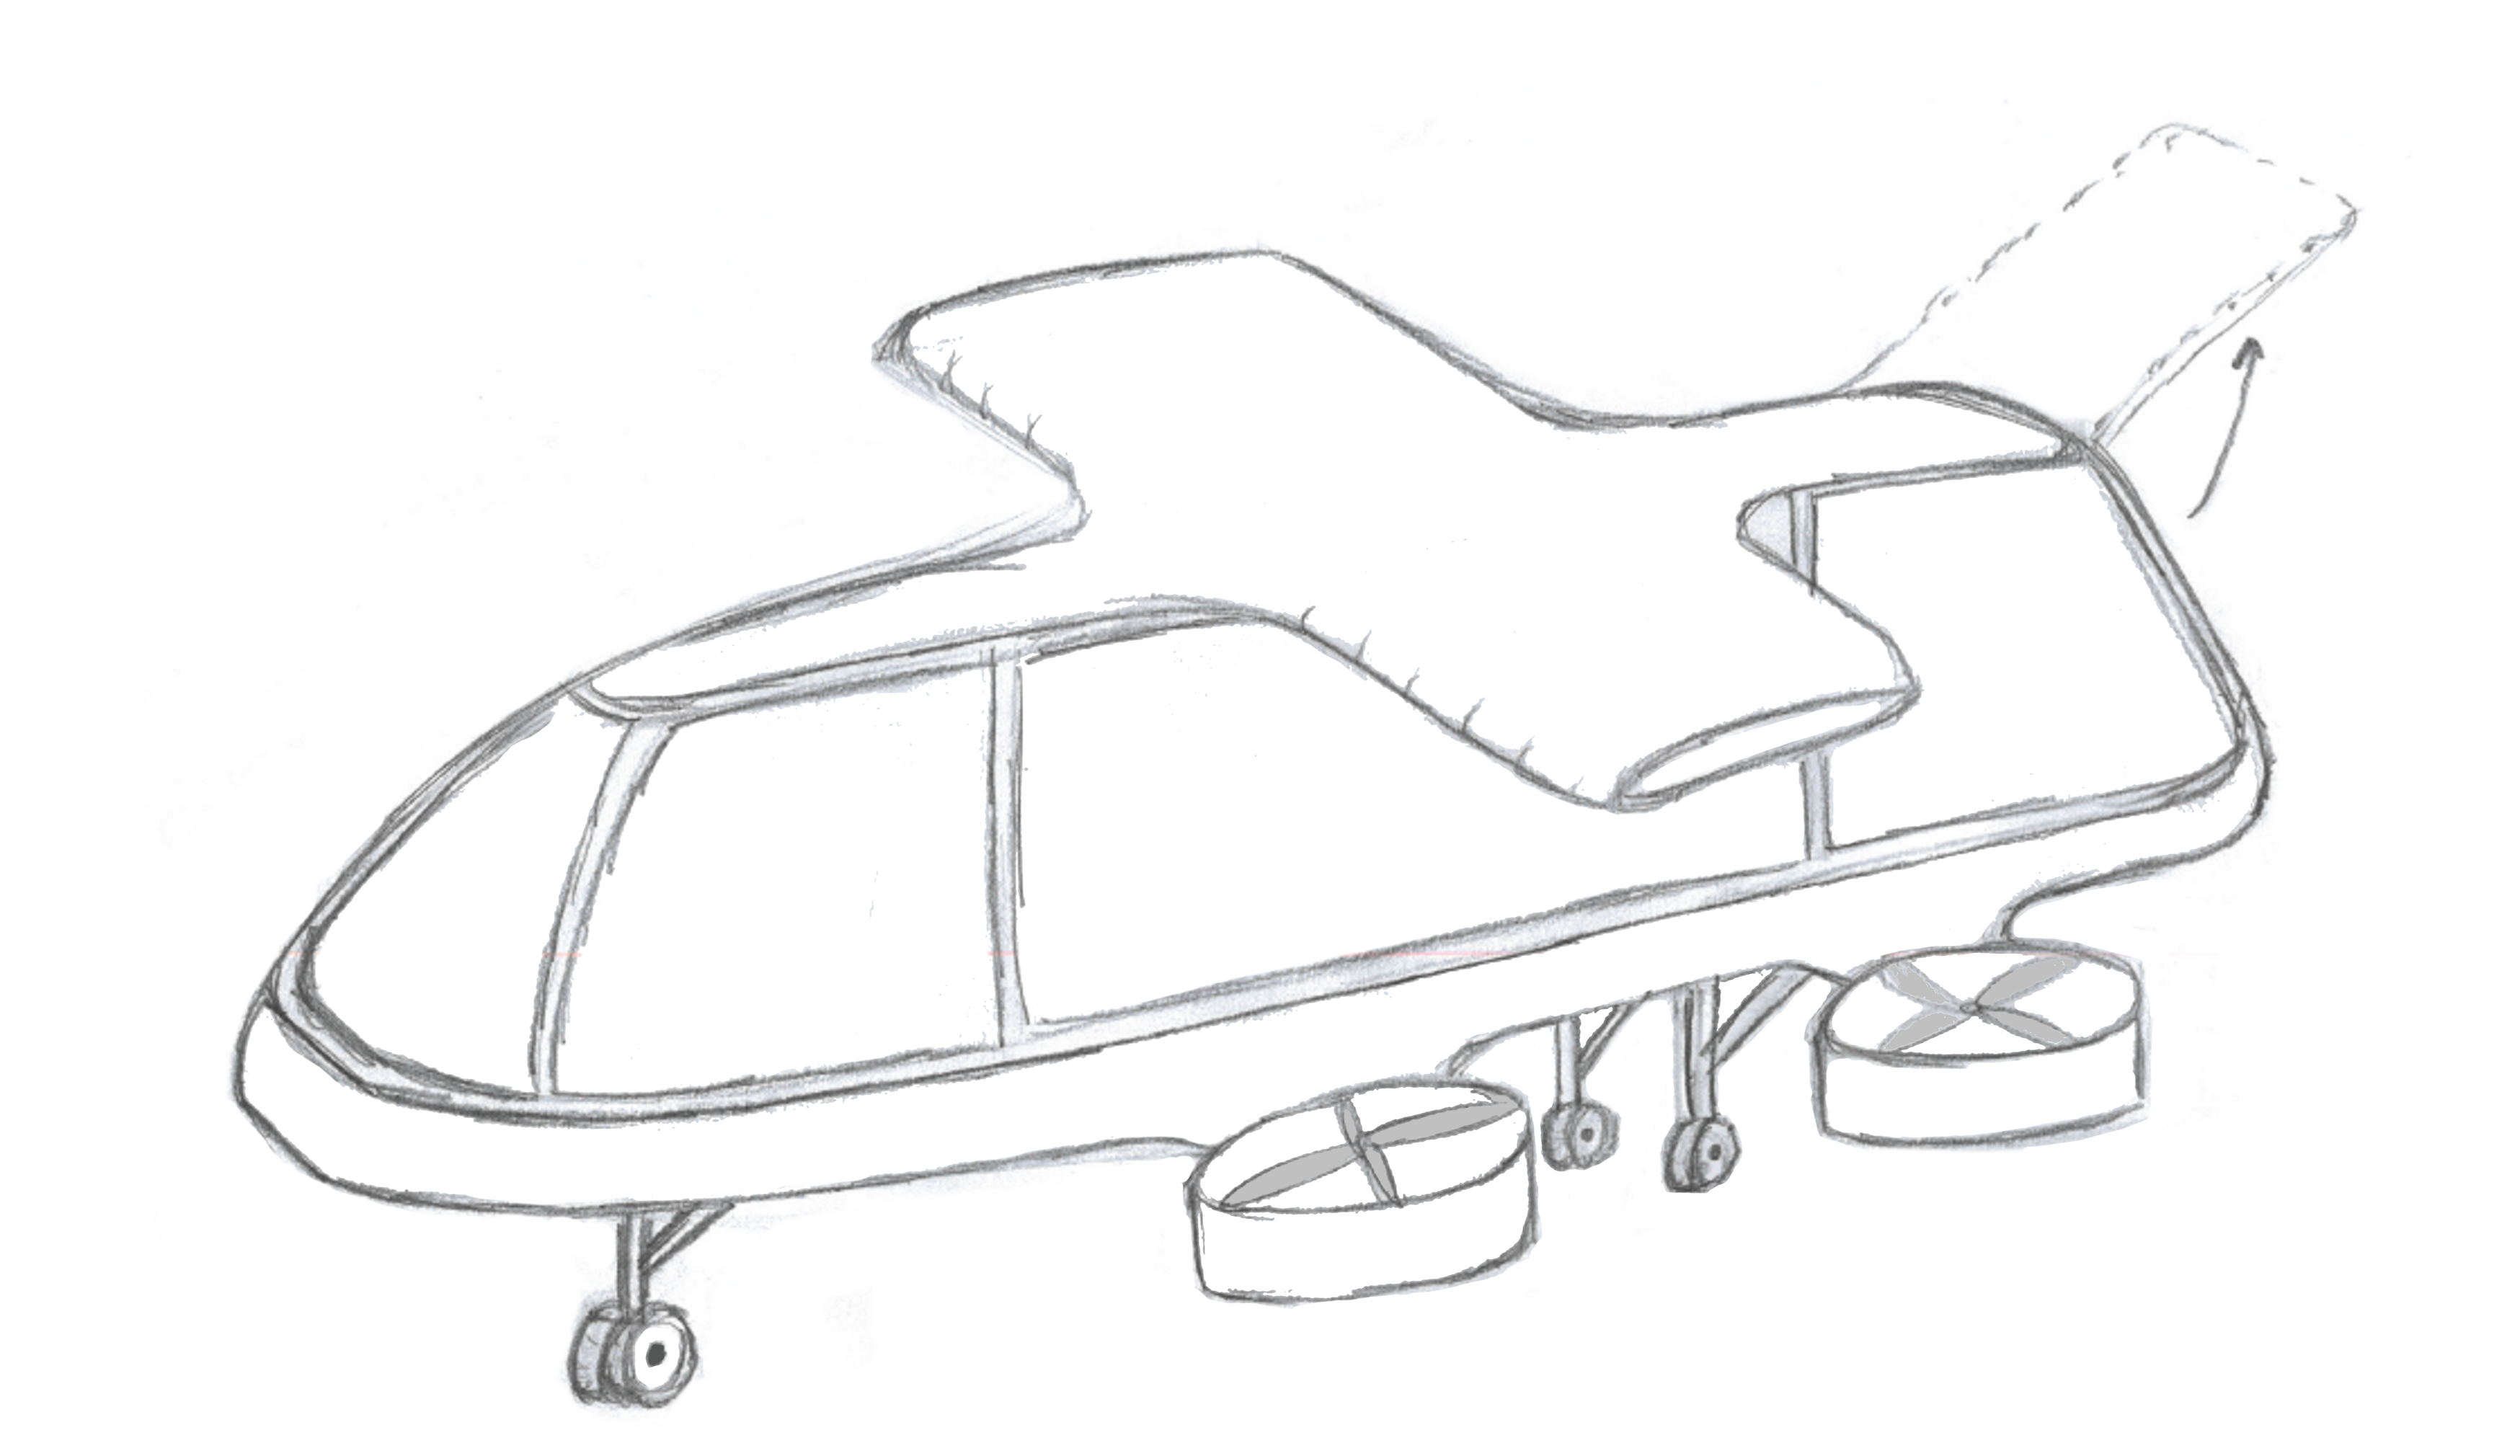
\includegraphics[width=5.0cm]{./Figures/Concept_20A.png}
    \captionsetup{justification=centering}
    \caption{Concept 20A}
    \label{concept20a}
  \end{minipage}
  \hspace{1.25cm}
  \begin{minipage}[b]{0.25\textwidth}
    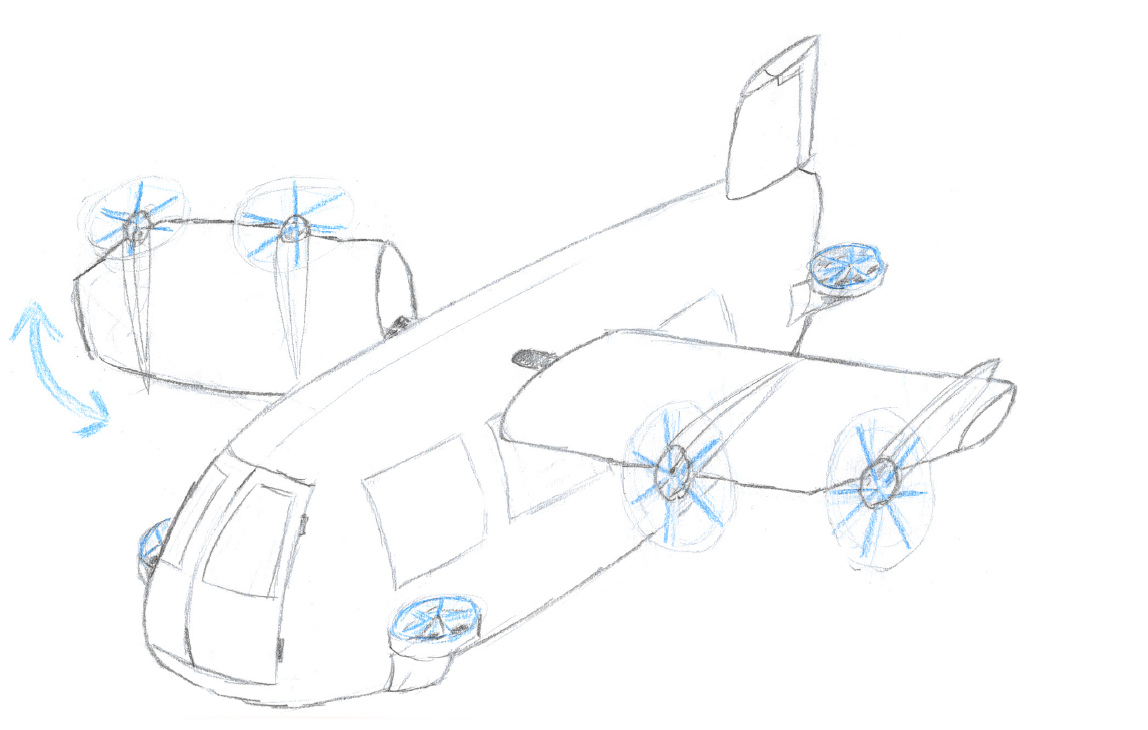
\includegraphics[width=5.0cm]{./Figures/Concept_20B.png}
    \captionsetup{justification=centering}
    \caption{Concept 20B}
    \label{concept20b}
  \end{minipage}
  \hspace{1.25cm}
  \begin{minipage}[b]{0.25\textwidth}
    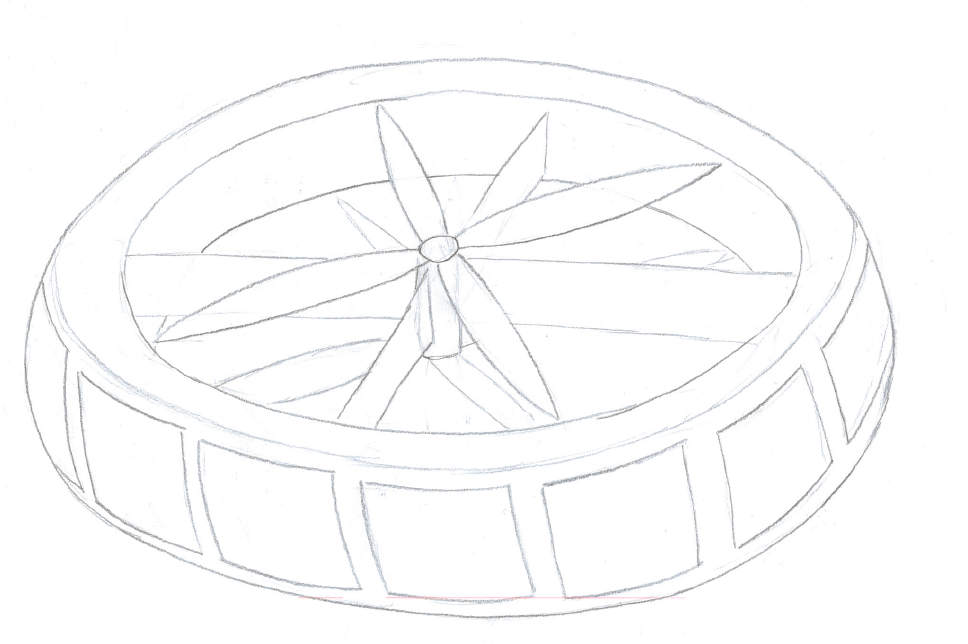
\includegraphics[width=5.0cm]{./Figures/Concept_20D.png}
    \captionsetup{justification=centering}
    \caption{Concept 20C}
    \label{concept20c}
  \end{minipage}
\end{figure}

\paragraph{Concept 20A}
Concept 20A features both a fixed wing and tilting rotors. The passengers enter the vehicle through the back and sit in a 3 abreast configuration, with a total of 7 rows. During take-off, the 4 propellers provide the thrust for VTOL and, at a specified height, they will rotate to provide the thrust and part of the lift during cruise. The vehicle will land on a set of wheels in tricycle configuration and can then be plugged in for charging. The battery of the vehicle will be under the floor of the passengers. More details on this vehicle concept can be found in \autoref{20input}.  

\paragraph{Concept 20B}
Concept 20B is a tilt wing concept. The passengers enter through the front of the aircraft and sit 4 abreast in a one-aisle configuration. There will be 5 rows to accommodate 20 passengers. It features 4 rotors on the wings and 2 mounted to the back and front of the fuselage respectively to provide stability, resulting in a total of 8 rotors. All of these rotors will be used during take-off, landing and hover. During the cruise phase, the wings will tilt such that the propellers provide thrust and the wings provide all the lift needed for flight. The smaller rotors at the front and rear of the aircraft will be predominantly used for the longitudinal stability. The landing gear and battery will, as in concept 1, be located under the the floor, in the belly of the vehicle. Extra room for batteries is available in the back. More details on this vehicle concept can be found in \autoref{20input}.  

\paragraph{Concept 20C}
Concept 20C is a design that is quite different compared to the ones seen so far. It is a coaxial rotor surrounded by a passenger compartment. The passengers will be seated in a circle configuration around this rotor facing outwards. The large rotor will provide the lift, thrust and stability. The battery will be located under the floor of the cabin and in the structure that holds the rotor in place. The latter will cause a bending relief.  Again, more details on this vehicle concept can be found in \autoref{20input}.  

The three options are summarised in table \autoref{20input}. They will be plugged into the tool with the goal of comparing the different concepts in this vehicle class at a later stage. 

\begin{table}[H]
\centering
\captionsetup{justification=centering}
\caption{Input of tools for 20+ person vehicle}
\label{20input}
\begin{tabular}{@{}llll@{}}
\toprule
\textbf{Parameter}                       & \textbf{Concept 20A} & \textbf{Concept 20B} & \textbf{Concept 20C} \\ \midrule
MTOW {[}kg{]}                            &    9000                &       7000             &  12000                  \\
OEW/MTOW           &        0.45            &           0.45         &      0.40              \\
\# Passengers {[}-{]}                    &        21            &        20            &       20             \\
Range {[}km{]}                           &        60            &        60            &           20         \\
Max Dimension {[}m{]}                    &          18         &        18            &          16          \\
%Battery Energy density {[}Wh/kg{]}       &         260            &     260               &       250             \\
%Battery Power density {[}W/kg{]}         &           2100        &        2100            &         2500           \\
L/D {[}-{]}                              &         8.0           &        13            &     2               \\
Radius of rotors (x number of rotors)  &           2.5 (x4)         &   1.85 (x4), 0.85 (x4)                 &     6 (1x)               \\
Cruise Velocity {[}m/s{]}                &          83          &        111           &  42                 \\ \bottomrule
\end{tabular}

\end{table}


\subsection{Intermediate Trade-off}
\label{InterTO-20}
%Present the outputs of the tools for each option, put it in a table and discuss which 1 (or 2) is best. Explain that we will continue with that one to the final trade off, where we will investigate that option further by looking at additional qualitative factors like user experience, passenger comfort, safety etc.. 

As mentioned before, the inputs that were specified in \autoref{ssc:Conceptdef20} are fed to a tool that computes some outputs which will be the basis for comparing the concepts in this vehicle class.  


% \begin{table}[H]
% \centering
% \captionsetup{justification=centering}
% \caption{Output of tools for 20+ person vehicle}
% \label{20output}
% \begin{tabular}{@{}llll@{}}
% \toprule
% \textbf{Parameter}                           & \textbf{Concept 20A} & \textbf{Concept 20B} & \textbf{Concept 20C} \\ \midrule
% \# Vehicles {[}-{]}                          &       1600             &     1500            &      1700                 \\
% \# Pads {[}-{]}                              &         570           &      550           &          645            \\
% \# Trips/day {[}-{]}                         &         25800           &       26000          &         20000               \\
% \#  Payload Range Energy Efficiency           &        0.0164           &       0.0226         &         0.00538            \\
% \# Ticket price per kilometre {[}\$/(km){]} &           7.81           &          7.84       &        13.70               \\
% \# Ticket price {[}\$/km-pad costs{]}        & 0.63                    &      0.59            &   --            \\
% \# Passengers/day {[}-{]}                    &         268000           &       259000          &      209000               \\
% Vertiport Area {[}m\textsuperscript{2}{]}    &           5700         &        5700         &        4600              \\
% Total System Area {[}km\textsuperscript{2}{]} &       3.23             &      3.12           &       2.94               \\
% Total Board Time {[}s{]}                     & 1065                   &     1020            &      1020                \\
% Noise {[}dBA{]}                              &           89        &      89           &       94                  \\
% Downwash {[}m/s{]}                              &             45       &     48          &  --   \\ 
% Maximum Hub Throughput [vehicles/hour]      & 1135    & 1155 & -- \\ \bottomrule
% \end{tabular}

% \end{table}

\begin{table}[h]
\centering
\captionsetup{justification=centering}
\caption{Output of tools for 20+ person vehicle}
\label{20output}
\begin{tabular}{@{}llll@{}}
\toprule
\textbf{Parameter}                                          & \textbf{Concept 20A} & \textbf{Concept 20B} & \textbf{Concept 20C} \\ \midrule
\# Vehicles                                                 &      1600             &     1500            &      1700         \\
Payload Range Energy Efficiency    {[}-{]}                      &      0.0164           &       0.0226         &         0.00538         \\
Ticket price {[}\$/km-pad costs{]}                          &   0.63                    &      0.59            &   --           \\
\# Passengers/day {[}-{]}                                   &     268000           &       259000          &      209000     \\
Total System Area {[}m\textasciicircum{}2                   &    3.23             &      3.12           &       2.94      \\
Noise {[}dBA{]}                                             &      89        &      89           &       94       \\ 
Downwash {[}m/s{]}                                          &      45       &     48          &  --  \\ \bottomrule
\end{tabular}
\end{table}

\autoref{20criteriascores} shows the resultant criteria scores for concepts 20A and 20B. Concept 20C is limited in the fact that several output parameters, including the down-wash and the ticket price, did not converge or were nonsensical. With the lack of output parameters, the concepts were not able to be properly assessed against the criteria, hence only concepts 20A and 20B are further evaluated. 

\begin{table}[h]
\captionsetup{justification=centering}
\caption{Criteria scores for 20 person vehicle}
\label{20criteriascores}
\begin{tabular}{@{}lllll@{}}
\toprule
\textbf{Group}         &  \textbf{Criteria}         & \textbf{Criteria Weight}         & \textbf{Concept 20A} & \textbf{Concept 20B}      \\  \midrule
\multirow{2}{*}{Ecologic Sustainability} & PREE & 0.278                   & 1             & 3                  \\
                                         & Battery mass       & 0.078                   & 1             & 3                  \\\midrule
\multirow{2}{*}{Social Acceptance}       & Noise              & 0.258                   & 2             & 2                \\
                                         & Downwash           & 0.055                   & 4             & 4           \\\midrule
Cost/Profit                              & Ticket price       & 0.189                   & 2             & 2                  \\\midrule
Technical Risk                           & ATM/UTM efforts    & 0.140                   & 3.22          & 2.87                  \\  \midrule
\textbf{}                                & \textbf{}          & \textbf{Weighted Score} & \textbf{1.92} & \textbf{2.59}  \\ \bottomrule
\end{tabular}
\end{table}

From \autoref{20criteriascores}, it can be seen that concept 20B is the best to proceed with, having a top weighted score of 2.59. Comparing concepts 20A and 20B, it can be seen that the two concepts have very similar parameter values in areas such as noise, passengers per day and ticket price. The main criterion in which the two differ is in ecologic sustainability, where concept 20B  has a very reduced battery mass and has a significantly higher PREE. Therefore concept 20B  will be investigated further in \autoref{Sec:FinalTO}.  


% moved to VandV section


\section{Final Trade-off}
\label{Sec:FinalTO}
%Present qualitative aspects for each final concept
%run the final trade off
%present the final 
Now that the most feasible option for each vehicle passenger range has been selected, they will be compared with each other. For clarity, an overview of the inputs and outputs of the winning concepts in each category are shown below in \autoref{inputswin} and \autoref{outputswin} respectively. 

\begin{table}[H]
\centering
\captionsetup{justification=centering}
\caption{Inputs of winning vehicles}
\label{inputswin}
\begin{tabular}{llll}
\hline
\textbf{Parameter}                    & \textbf{1-2 pax}      & \textbf{4-6 pax} & \textbf{20+ pax}    \\ \hline
MTOW {[}kg{]}                         & 575                   &    971              & 7418                \\
OEW/MTOW        & 0.40                    &   0.35          & 0.45                  \\
\# Passengers {[}-{]}                 & 2                     &      4            & 20                  \\
Range {[}km{]}                        & 60                    &       60           & 60                  \\
Max Dimension {[}m{]}                 & 5                     &      10            & 18                  \\
%Battery Energy density {[}Wh/kg{]}    & 260                &      260            & 260               \\
%Battery Power density {[}W/kg{]}      & 2100               &          2100        & 2100              \\
L/D {[}-{]}                           & 12                    &       15           & 13                  \\
Radius of rotors (x number of rotors) & 0.85 (2x) \& 0.8 (2x) &    1 (x4); 1.5 (x1); 0.7 (x2)             & 2.5 (x4), 0.85 (x4) \\
Cruise Velocity {[}m/s{]}             & 32                    &        82          & 111.1               \\ \hline
\end{tabular}
\end{table}

% \begin{table}[H]
% \centering
% \captionsetup{justification=centering}
% \caption{Outputs of winning vehicles}
% \label{outputswin}
% \begin{tabular}{llll}
% \hline
% \textbf{Parameter}                          & \textbf{1-2 pax} & \textbf{4-6 pax} & \textbf{20+ pax} \\ \hline
% \# Vehicles {[}-{]}                         & 12900             &     3350             & 1500             \\
% \# Pads {[}-{]}                             & 1620             &        800          & 550              \\
% \# Trips/day {[}-{]}                        & 308000           &       124000           & 26000            \\
% \# PREE {[}Wh/(pax-km){]}                   & 0.0352           &       0.0415          & 0.0226           \\
% \# Ticket price per kilometre {[}\$/km{]} & 2.34             &    3.85              & 7.84             \\
% \# Ticket price per kilometre {[}\$/km - pad costs{]} & 0.62             &    0.42              & 0.59             \\
% \# Passengers/day {[}-{]}                   & 32700           &     269000             & 259000           \\
% Vertiport Area {[}m\textsuperscript{2}{]}   & 630            &     2870             & 5700             \\
% Total System Area {[}km{]}\textsuperscript{2}  & 1.01          &       1.55           & 3.12          \\
% Total Board Time {[}s{]}                    & 210              &        300          & 1020             \\
% Noise {[}dBA{]}                             & 71             &       74           & 89             \\ 
% Downwash [m/s]                              & 51            &       33              &   48      \\
% Maximum Hub Throughput [vehicles/hour]      & 16389    & 5816 & 1155 \\ \hline
% \end{tabular}
% \end{table}

\begin{table}[h]
\centering
\captionsetup{justification=centering}
\caption{Output of winning vehicles}
\label{outputswin}
\begin{tabular}{@{}llll@{}}
\toprule
\textbf{Parameter}                                          & \textbf{1-2 pax} & \textbf{4-6 pax} & \textbf{20+ pax}  \\ \midrule
\# Vehicles                                                 &      12900             &     3350             & 1500       \\
Payload Range Energy Efficiency    {[}-{]}                      &     0.0352           &       0.0415          & 0.0226          \\
Ticket price {[}\$/km-pad costs{]}                          &   0.62             &    0.42              & 0.59       \\
\# Passengers/day {[}-{]}                                   &    32700           &     269000             & 259000      \\
Total System Area {[}m\textasciicircum{}2                   &    1.01          &       1.55           & 3.12    \\
Noise {[}dBA{]}                                             &      71             &       74           & 89      \\ 
Downwash {[}m/s{]}                                          &      51            &       33              &   48  \\ \bottomrule
\end{tabular}
\end{table}


In \autoref{sec:Criteria} the trade-off criteria, according to which the concepts will be scored, were explained. The corresponding weight factors for all the criteria are tabulated in \autoref{subsec:weights}. 
% For all of the criteria a scale from 1 to 5 was created to normalise the absolute values of the parameters. The weighted score for the quantitative criteria were then easily calculated by placing the quantitative values in the range of set values, where each range belongs to a score. For the qualitative criteria, each team member gave a score from 1 to 5 to each of the concepts. The average score of each concept was then weighted by the established weight factors. Due to the different opinions of the team members an average score is produced, thus for the qualitative factors decimal scores are produced rather than integers. The concept with the highest score is the winning concepts. In \autoref{TO-summary} the trade-off summary table is shown. The highest score for each criteria is highlighted in green.
From this table it becomes apparent that the 4-6 pax concept is the winning concept. Designing this winning concept in more detail and determining the corresponding infrastructure and system layout will be the focus of the final phase of the DSE. 

% Please add the following required packages to your document preamble:
% \usepackage[table,xcdraw]{xcolor}
% If you use beamer only pass "xcolor=table" option, i.e. \documentclass[xcolor=table]{beamer}
\begin{table}[H]
\centering
\captionsetup{justification=centering}
\caption{Trade-off summary table}
\label{TO-summary}
\begin{tabular}{lcccc}
\hline
\multicolumn{1}{c}{\textbf{Criteria}} & \multicolumn{1}{l}{\textbf{Total Weights}} & \multicolumn{1}{r}{\textbf{2 pax}} & \multicolumn{1}{l}{\textbf{4-6 pax}} & \multicolumn{1}{l}{\textbf{20 pax}} \\ \hline
PREE & 0.278 & \cellcolor[HTML]{E6FFE5}5 & \cellcolor[HTML]{E6FFE5}5 & 3 \\
Battery mass & 0.078 & 4 & \cellcolor[HTML]{E6FFE5}5 & 3 \\
Safety & 0.185 & 2.9 & \cellcolor[HTML]{E6FFE5}3.3 & 2.5 \\
Passenger experience & 0.056 & \cellcolor[HTML]{E6FFE5}4.1 & 3.7 & 2.7 \\
Noise & 0.055 & \cellcolor[HTML]{E6FFE5}5 & \cellcolor[HTML]{E6FFE5}5 & 2 \\
Downwash & 0.017 & \cellcolor[HTML]{E6FFE5}5 & \cellcolor[HTML]{E6FFE5}5 & 4 \\
Development cost & 0.036 & \cellcolor[HTML]{E6FFE5}4 & 3 & 1.8 \\
Ticket price & 0.153 & 2 & \cellcolor[HTML]{E6FFE5}5 & 2 \\
ATM/UTM efforts & 0.081 & 1.4 & 2.7 & \cellcolor[HTML]{E6FFE5}2.9 \\
Weather conditions & 0.043 & 2.1 & 2.7 & \cellcolor[HTML]{E6FFE5}3.7 \\
Modification of regulations & 0.018 & \cellcolor[HTML]{E6FFE5}3.7 & 3 & 1.5 \\ \hline
\multicolumn{2}{c}{\textbf{Sum of Weighted Scores}} & \cellcolor[HTML]{FFFC9E}\textbf{3.55} & \cellcolor[HTML]{67FD9A}\textbf{4.22} & \cellcolor[HTML]{FD6864}\textbf{2.65} \\ \hline
\end{tabular}
\end{table}

%Naturally, this list of quantitative parameters is not the complete picture. There are other factors of a potential UAM system that are of relevance too. They are the ones that are of qualitative nature and have therefore not been examined in the tool. The factors that are looked at are the safety, the passenger experience, the ATM/UTM efforts needed, the susceptibility to harsh weather conditions and the modifications that would have to be done to the current regulations for a system to work. Each of these five factors will be given a score in the range from 1-5 and, after which this number is multiplied with the weight that was assigned to it in \autoref{subsec:weights}. A weighted average is computed for each of the concepts. All of the aforementioned can be found in table (REF TO TABLE) below. 

%THE ULTIMATE TABLE!!!!! THIS INCLUDES OUR CRITERIA WITH THEIR WEIGHTS AND THE SCORE THAT THEY GET. INCLUDE A WEIGHTED AVERAGE FOR EACH OF THE CONCEPTS AND THERE WE HAVE IT: ---> OUR WINNING CONCEPT <--- 


\section{Risk Analysis}
\label{sc:RiskAnalysis}
The implementation of a new transport system brings along several risks. They will be outlined in \autoref{subsec:ri}. In \autoref{sec:riskmit}, several mitigation strategies are described for the most crucial risks. 


\subsection{Risk Identification}
\label{subsec:ri}
Some of the more crucial risks have been identified an are listed below. The first list gives an overview of the vehicle risks. 

\begin{enumerate}[nolistsep]
    \item The structural percentage is underestimated. This results in a higher structural mass; this snowballs in a higher MTOW 
    \item Noise levels are too high for the system to be implemented in an urban environment 
    \item The technology needed to fly the vehicles autonomously is not mature enough yet 
    \item There is a battery fire during flight
    \item There is bird-strike when the vehicle is in flight 
    \item The tilt-wing mechanism fails and the vehicle is unable to change the orientation of the wing 
    \item The required structural layout compromises the user experience in terms of space and windows 
    \item The required size of the canard to ensure longitudinal stability is large, resulting in a loss of efficiency 
    \item One or more propellers fail, leading to reduced stability 
\end{enumerate}

The list below is an overview of the operational risks. 

\begin{enumerate}[resume, nolistsep]
    \item ATM system not developed yet in order to accommodate UAM system.
    \item The concept is not economically feasible 
    \item Society is not yet confident in the level of safety of UAM system.
    \item No improvement in battery charge rate density is realised. This will increase the charge time of the aircraft
    \item The number of charge/discharge cycles for batteries is not commensurate with the life time of the vehicle 
    \item There is limited airspace available to conduct operations 
    \item The regulations in 2050 do not allow the usage of UAM vehicles yet.
    \item There is a labour strike
    \item The city has no space available to accommodate the number of vertiports needed for operations 
    \item Climate change has lead to more severe weather conditions 
    \item The required modifications to the grid are either impossible to realise or too expensive to implement
\end{enumerate}


\subsection{Risk Mitigation}
\label{sec:riskmit}
The following risk mitigation strategies are applied to mitigate the high ranking risks: 

\begin{itemize}[nolistsep]
    \item Risk 4: Ensure the fire is contained by building a protective casing around the battery. This protective casing should be tested to ensure it is of sufficient quality. The passengers must be made aware of the emergency procedures.
    \item Risk 5: The probability of occurrence cannot be changed, however, the vehicle can be designed such that the consequences of a bird strike are less.
    \item Risk 6: The probability of occurrence cannot be changed, however, landing wheels shall be added to make a horizontal landing possible as well.
    \item Risk 8: The size of the canard can be reduced by shifting the centre of gravity of the vehicle more aft.
    \item Risk 11: The business model can consider a smaller and wealthier target group.
    \item Risk 12: Promote UAM safety awareness through advertisements and demonstrations.
    \item Risk 13 \& 14: The option to use swapable batteries should be available until the detailed design phase. Doing this will enable the system to have very quick turnaround time.
    \item Risk 15: The route networks has to be adjusted in such a way that airspace needed does not interfere with flight-path.
    \item Risk 18: In case the required system area is too big, the market share could be reduced. This would lead to a reduced number of vertiports.
    \item Risk 20: The charge rate of the batteries could be decreased, however, this could mean that more vehicles would be needed to achieve the same number of transported people. A second option is to choose to go for a smaller market share. In case of the latter, the breakeven point will be set back. This is assumed to be less of a risk to the project.

\end{itemize}

All these mitigation strategies are essential but will move you away from the ideal business strategy. Two risk maps are shown in \autoref{fig:riskmap123}, they show the risks mentioned before in a chart before and after risks mitigation. 

\begin{figure}[H]
    \centering
    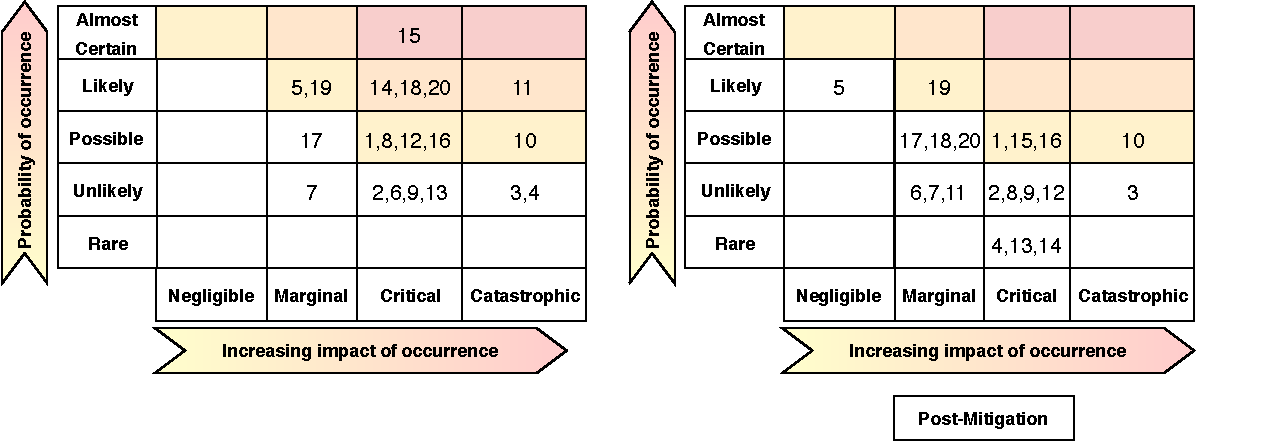
\includegraphics[width = \linewidth]{Figures/riskmap.pdf}    
    \caption{Risk map before and after risk mitigation}
    \label{fig:riskmap123}
\end{figure}


